% ----------------------------------------------------------
\chapter{Desenvolvimento do Projeto}
% ----------------------------------------------------------

Depois das definições apresentadas e da escolha de componentes apresentada na seção anterior, foi possível construir um esquemático elétrico, que esquematiza a PCB do OBDH. Nesse capítulo, discutir-se-á circuitos específicos mais relevantes do projeto, usando o esquemático pronto, que se encontra no Anexo I.

\section{Conversores de Potência}

Partindo do princípio que o módulo EPS da terceira geração de módulos do SpaceLab será capaz de fornecer 3,3 V para o OBDH, foi proposta uma cascata de potência descrita na Figura \ref{fig:power}. Nela, são suprimidos os circuitos de proteção que serão descritos posteriormente.

\begin{figure}[H]
    \centering
    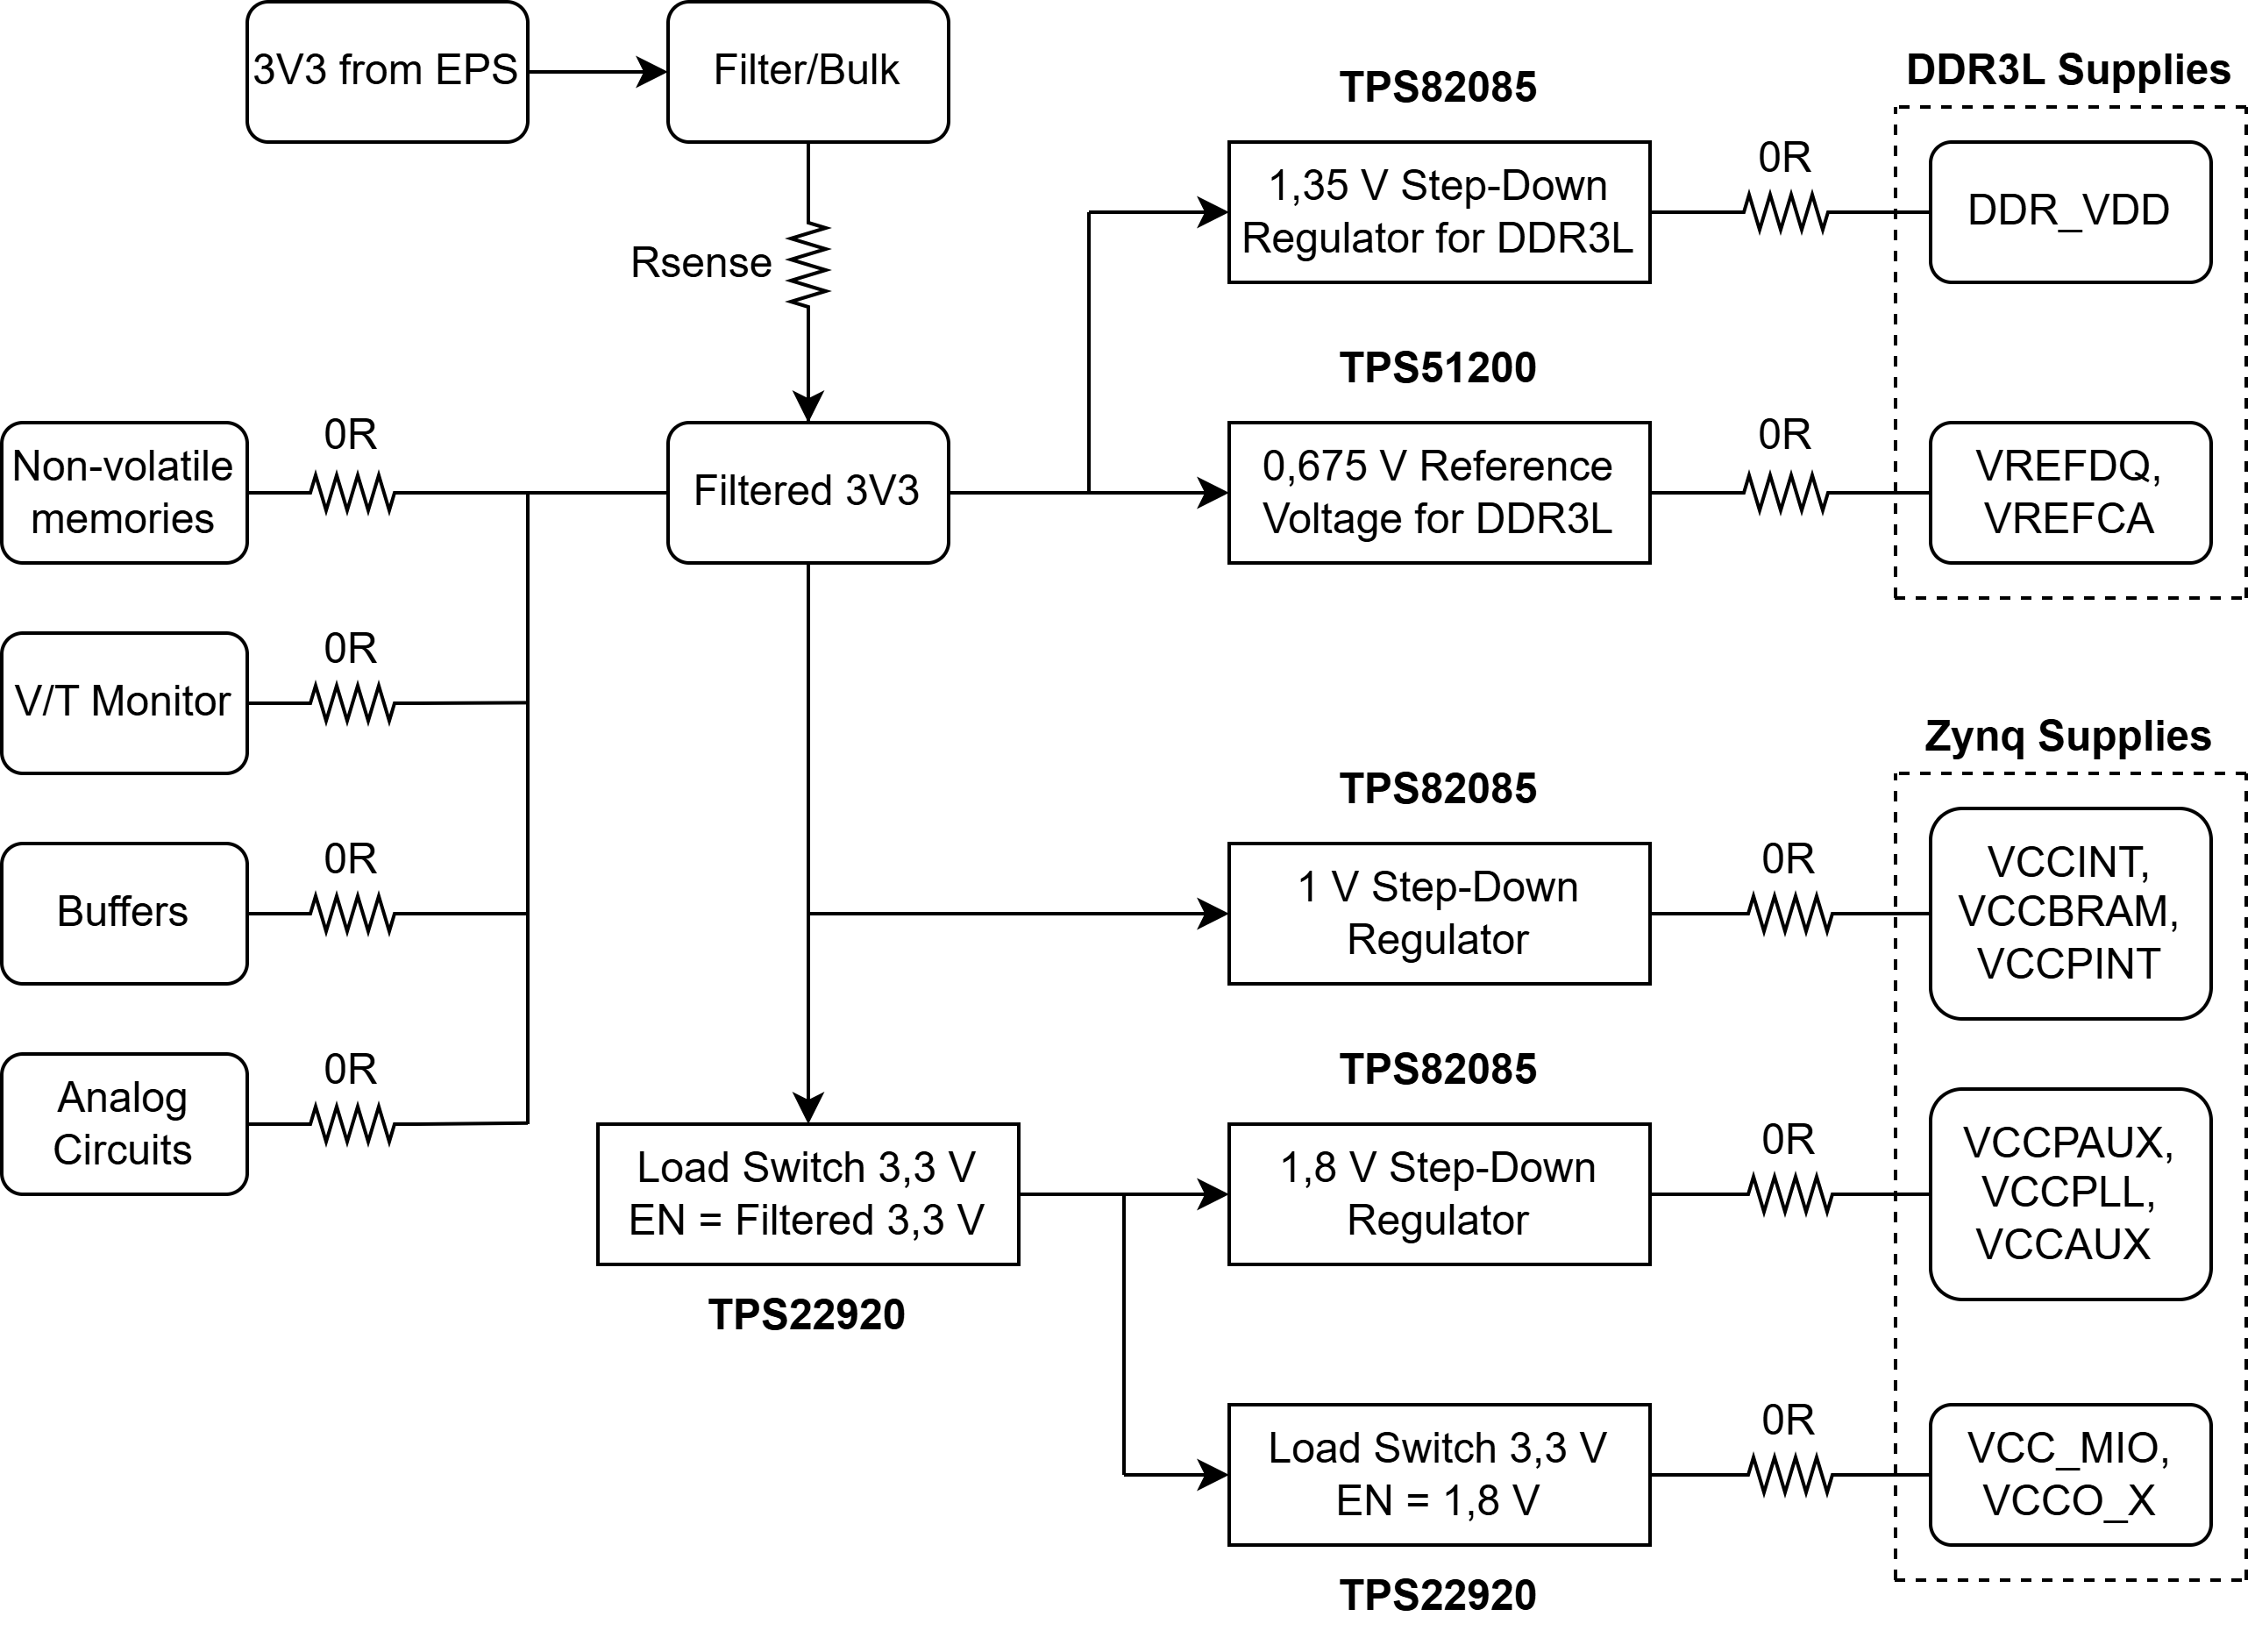
\includegraphics[scale=0.6]{images/Power_system.png}
    \caption{Cascata de potência proposta.}
    \label{fig:power}
    \fonte{Elaboração própria.}
\end{figure}

\subsection{Filtro de Entrada}

Costumeiramente, a entrada de tensão de uma placa robusta deve ser filtrada, principalmente devido às flutuações do ruído conduzido de outros subsistemas do satélite, caracterizando o fenômeno de Interferência Eletromagnética (EMI), esquematizado na Figura \ref{fig:emi}.

\begin{figure}[H]
    \centering
    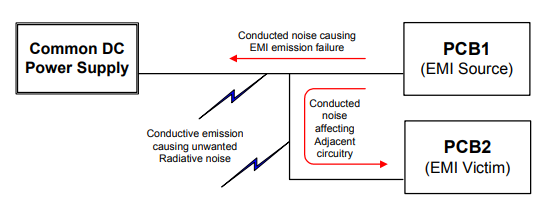
\includegraphics[scale=1]{images/EMI noise.png}
    \caption{Interferência com ruído conduzido.}
    \label{fig:emi}
    \fonte{SOH et al., 2010.}
\end{figure}

Além disso, também foi necessária a inclusão de um diodo Zener em paralelo à entrada, servindo como um elemento extra de proteção contra perturbações e transientes (CADENCE, 2023). Outra característica explorada foi a colocação de capacitores em paralelo, a fim de reduzir sua resistência em série equivalente (ESR) e sua indutância série (SARJEANT, 1990).  O filtro proposto está disposto na Figura \ref{fig:FILTRO}.  Além disso, sua magnitude e fase simuladas estão dispostas na Figura \ref{fig:filtrof}.

\begin{figure}[H]
    \centering
    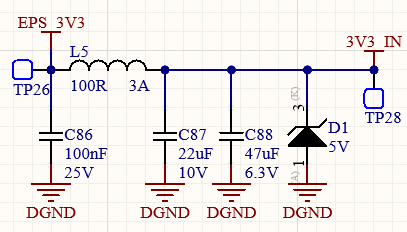
\includegraphics[scale=1]{images/FILTRO.png}
    \caption{Filtro proposto.}
    \label{fig:FILTRO}
    \fonte{Elaboração própria.}
\end{figure}

\begin{figure}[H]
    \centering
    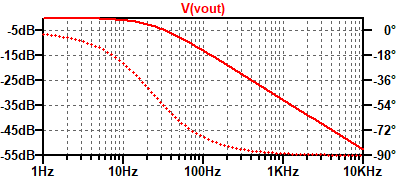
\includegraphics[scale=1]{images/filtrof.png}
    \caption{Simulação de magnitude e fase em função da frequência para o filtro proposto.}
    \label{fig:filtrof}
    \fonte{Elaboração própria.}
\end{figure}

\subsection{Cascata de potência}

Devido à escolha do SoC e da memória DDR3, foi necessária a definição de uma cascata de potência, levando-se em consideração os requisitos de (UG585, 2023), que descreve o sequenciamento das tensões para o menor consumo de potência e para garantir a integridade do fusível interno do SoC. Dessa forma, como pode-se ver na Figura \ref{fig:power}, são usados os denominados \textit{load switches}, a fim de garantir o sequenciamento descrito e garantir uma proteção efetiva contra sobrecorrente (MAK, 2018). 

O primeiro regulador, que gera a tensão de 1 V, apresentado na Figura \ref{fig:1vsupp}, é o primeiro da cascata. Seu divisor de tensão de saída foi calculado conforme (TPS82085, 2019):

\begin{equation}
	V_{out} = 0,8 * (1 + R_1/R_2) = 0,8 * (1+ 37,4k/150k) = 0,999 V
\end{equation} 

\begin{figure}[H]
    \centering
    \includegraphics[scale=0.8]{images/1vsupp.png}
    \caption{Regulador de tensão de 1 V.}
    \label{fig:1vsupp}
    \fonte{Elaboração própria com base no circuito apresentado pelo fabricante.}
\end{figure}

Também foi possível montar seu circuito de proteção de sobrecorrente, disposto na Figura \ref{fig:1vocp}. Seu resistor de entrada, que escolhe o limiar de corrente permitido, foi caculado conforme (LTC4361, 2018), considerando uma corrente 20\% superior à máxima calculada (na Tabela \ref{tab:estpow}):

\begin{equation}
	R_{sense} = 50 mV / I_{max} =50 / 2,63 = 19,01 m\Omega
\end{equation} 

\begin{figure}[H]
    \centering
    \includegraphics[scale=1]{images/1vocp.png}
    \caption{Proteção contra \textit{latch-up} para a tensão de 1 V.}
    \label{fig:1vocp}
    \fonte{Elaboração própria com base no circuito apresentado pelo fabricante.}
\end{figure}

Depois disso, para seguir com o sequenciamento requerido pelo SoC, precisa-se de um circuito de chaveamento de carga, apresentado na Figura \ref{fig:sw1}. Seu circuito é baseado no sugerido por (TPS22920, 2016), com seu ligamento sendo feito pela própria tensão de 3,3 V.

\begin{figure}[H]
    \centering
    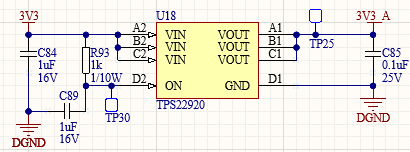
\includegraphics[scale=1]{images/sw1.png}
    \caption{Circuito de \textit{Load switch} para a tensão de 1,8 V.}
    \label{fig:sw1}
    \fonte{Elaboração própria com base no circuito apresentado pelo fabricante.}
\end{figure}

Analogamente, para a tensão de 1,8 V, são necessários ambos um conversor e um circuito de proteção. Estes estão dispostos respectivamente nas Figuras \ref{fig:1v8supp} e \ref{fig:1v8ocp} a seguir, conjuntamente com suas equações (3) e (4) para obtenção das resistências requeridas, usando a mesma margem de 20\% de corrente máxima. 

\begin{equation}
	V_{out} = 0,8 * (1 + R_1/R_2) = 0,8 * (1+ 110k/88,7k) = 1,792 V
\end{equation} 

\begin{figure}[H]
    \centering
    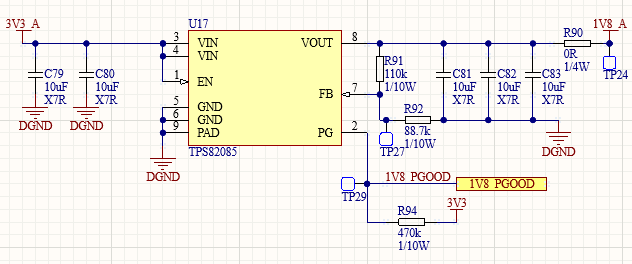
\includegraphics[scale=0.8]{images/1v8supp.png}
    \caption{Regulador de tensão de 1,8 V.}
    \label{fig:1v8supp}
    \fonte{Elaboração própria com base no circuito apresentado pelo fabricante.}
\end{figure}

\begin{equation}
	R_{sense} = 50 mV / I_{max} =50 / 0,5 = 100 m\Omega
\end{equation} 

\begin{figure}[H]
    \centering
    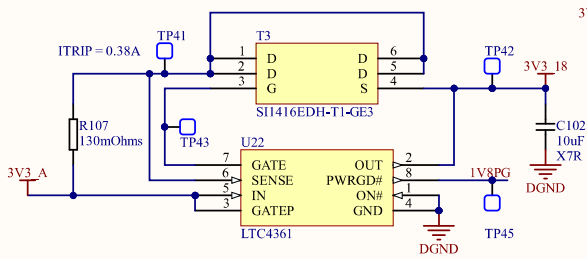
\includegraphics[scale=1]{images/1v8ocp.png}
    \caption{Proteção contra \textit{latch-up} para a tensão de 1,8 V.}
    \label{fig:1v8ocp}
    \fonte{Elaboração própria com base no circuito apresentado pelo fabricante.}
\end{figure}

Por fim, para ligar a tensão de 3,3 V fornecida para o SoC, é necessário um último circuito de chaveamento, dessa vez com seu ligamento feito pela tensão de 1,8 V, como mostra a Figura \ref{fig:sw2}.

\begin{figure}[H]
    \centering
    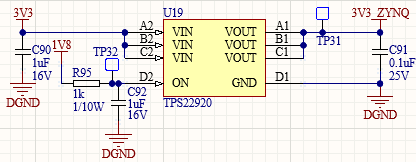
\includegraphics[scale=1]{images/sw2.png}
    \caption{Circuito de \textit{Load switch} para a tensão de 3,3 V do SoC.}
    \label{fig:sw2}
    \fonte{Elaboração própria com base no circuito apresentado pelo fabricante.}
\end{figure}

Paralelamente, para a memória DDR3L, são necessários um conversor para a alimentação, de 1,35 V, e um conversor para a tensão de referência e de terminação. Esses circuitos estão dispostos respectivamente nas Figuras \ref{fig:1v35supp} e \ref{fig:1v35ref}.

\begin{equation}
	V_{out} = 0,8 * (1 + R_1/R_2) = 0,8 * (1+ 47k/68k) = 1,353 V
\end{equation} 

\begin{figure}[H]
    \centering
    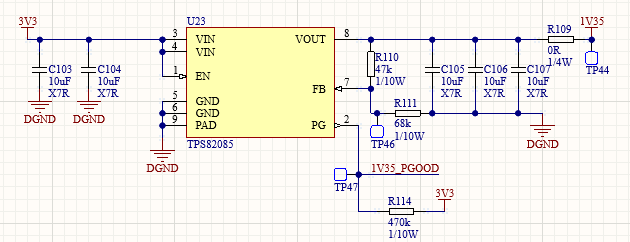
\includegraphics[scale=0.8]{images/1v35supp.png}
    \caption{Regulador de tensão de 1,35 V.}
    \label{fig:1v35supp}
    \fonte{Elaboração própria com base no circuito apresentado pelo fabricante.}
\end{figure}

\begin{figure}[H]
    \centering
    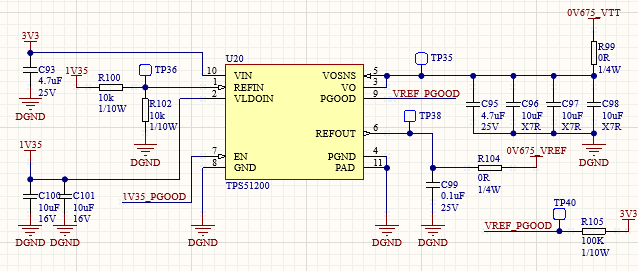
\includegraphics[scale=0.8]{images/refsupp.png}
    \caption{Regulador de tensão de referência e terminação para a memória DDR3L.}
    \label{fig:1v35ref}
    \fonte{Elaboração própria com base no circuito apresentado pelo fabricante.}
\end{figure}

\section{SoC}

No caso do SoC Zynq 7030, temos no total seis blocos operacionais, que incluem o funcionamento do PL e do PS, bem como as configurações e o bloco dedicado ao controlador da memória DDR (UG585, 2023). A seguir, estão dispostas as descrições funcionais e circuitos necessários para o funcionamento correto desse SoC, separados por cada um dos blocos citados.

\subsection{Bloco de Configuração}

O banco zero do SoC é o responsável por algumas opções e sinais de configuração. Abaixo, na Tabela \ref{tab:config}, se encontra a descrição funcional de cada pino desse banco, esquematizado na Figura \ref{fig:config}. Esse esquemático, bem como seus resistores de \textit{pull-up} (Figura \ref{fig:pullupconfig}), foram baseados na documentação técnica fornecida pela Xilinx (UG865, 2023) (UG470, 2023) (UG933, 2019) (DS191, 2018).


\begin{table}[H]
	\ABNTEXfontereduzida
	\caption{\label{tab:config}Descrição funcional dos pinos de configuração.}
	%\begin{tabular}{@{}p{2cm}p{2cm}p{2cm}p{2cm}p{2cm}p{2cm}p{3cm}@{}}
    \centering
    \begin{tabular}{@{} >{\centering}p{4cm} >{\centering}p{8cm} @{}}
    
		\toprule
		\textbf{Nome} & \textbf{Função} \tabularnewline 
        \midrule
         DXN e DXP & Terminais do diodo interno para medição de temperatura. \tabularnewline
         \midrule

         VREFP e VREFN & Tensões de referência do conversor analógico digital (XADC) do SoC. \tabularnewline

       \midrule
        VP e VN & Entrada extra do XADC. \tabularnewline

       \midrule
        VCCBAT & Não utilizada. Fonte da bateria. \tabularnewline

       \midrule
        TCK, TMS, TDI e TDO & Sinais da interface JTAG.  \tabularnewline

       \midrule
        INIT\_B & Indica inicialização da memória interna de configuração. \tabularnewline

       \midrule
       PROGRAM\_B & Reset assíncrono da lógica de configuração. \tabularnewline

       \midrule
        CFGBVS & Pino que seleciona o tipo de IO do banco 0. \tabularnewline

       \midrule
        DONE & Indica que a configuração foi terminada e feita corretamente. \tabularnewline

       \midrule
        VCCADC e GNDADC & Alimentação do XADC. \tabularnewline

       \midrule
        RSVDVCC e RSVDGND & Pinos de alimentação reservados. \tabularnewline

        \bottomrule
	\end{tabular}
	\fonte{Elaboração própria com base na documentação técnica do fabricante.}
\end{table}

\begin{figure}[H]
    \centering
    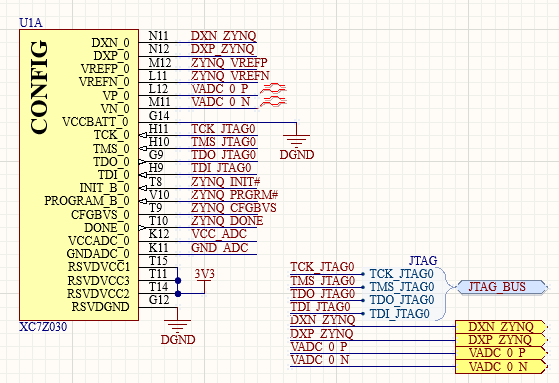
\includegraphics[scale=0.8]{images/zynqconfig.png}
    \caption{Banco de configuração do SoC.}
    \label{fig:config}
    \fonte{Elaboração própria com base no circuito apresentado pelo fabricante.}
\end{figure}

\begin{figure}[H]
    \centering
    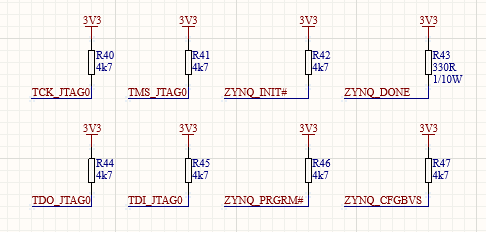
\includegraphics[scale=0.8]{images/pullupconfig.png}
    \caption{Resistores de \textit{pull-up} necessários.}
    \label{fig:pullupconfig}
    \fonte{Elaboração própria com base no circuito apresentado pelo fabricante.}
\end{figure}

Além disso, para a alimentação do XADC, foi necessário um circuito de filtragem, disposto na Figura \ref{fig:xadcfilter}, como requerido por (UG480, 2022).

\begin{figure}[H]
    \centering
    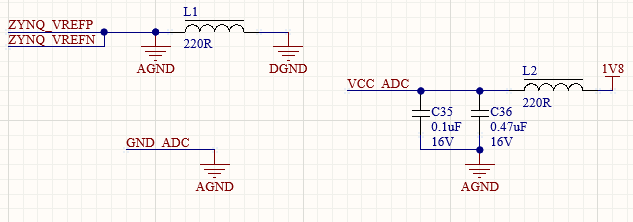
\includegraphics[scale=0.8]{images/xadcfilter.png}
    \caption{Filtro da alimentação analógica do SoC.}
    \label{fig:xadcfilter}
    \fonte{Elaboração própria com base no circuito apresentado pelo fabricante.}
\end{figure}


\subsection{Blocos do PS}

No caso do sistema de processamento (PS), temos dois bancos principais. O primeiro, denominado MIO (\textit{Multiplexed In-Out}), é onde se encontram os controladores das interfaces de comunicação, bem como a entrada de relógio e a escolha do \textit{boot}. No caso desse projeto, foi-se decidido que o SoC poderá inicializar de duas formas, sendo a primeira pela interface JTAG e a segunda pela memória Flash NOR (QSPI), escolhidos pelos resistores R48 e R51. O banco MIO e seus modos de inicialização estão dispostos nas Figuras \ref{fig:psmio} e \ref{fig:boot}. O outro banco do PS (112) não é utilizado nesse projeto.

\begin{figure}[H]
    \centering
    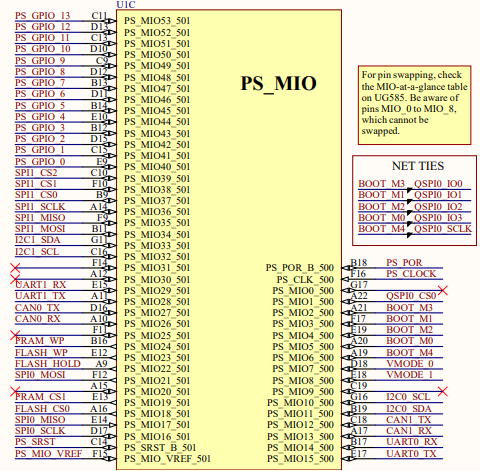
\includegraphics[scale=0.8]{images/psmio.png}
    \caption{Banco MIO do SoC com suas respectivas entradas e saídas.}
    \label{fig:psmio}
    \fonte{Elaboração própria com base na Tabela MIO-at-a-glance (UG585, 2023).}
\end{figure}

\begin{figure}[H]
    \centering
    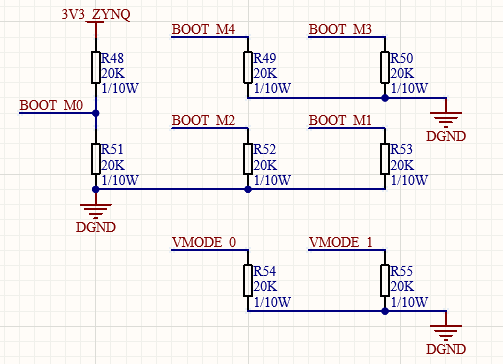
\includegraphics[scale=0.8]{images/bootmode.png}
    \caption{Modos de inicialização do SoC.}
    \label{fig:boot}
    \fonte{Elaboração própria com base em (UG585, 2023).}
\end{figure}

Por fim, Na Tabela \ref{tab:interfaces}, pode-se verificar qual a função de cada barramento de comunicação, em conformidade com a Figura \ref{fig:arq}. 

\begin{table}[H]
	\ABNTEXfontereduzida
	\caption{\label{tab:interfaces}Descrição das interfaces disponibilizadas.}
	%\begin{tabular}{@{}p{2cm}p{2cm}p{2cm}p{2cm}p{2cm}p{2cm}p{3cm}@{}}
    \centering
    \begin{tabular}{@{} >{\centering}p{4cm} >{\centering}p{8cm} @{}}
    
		\toprule
		\textbf{Interface} & \textbf{Função} \tabularnewline 
        \midrule
         SPI0 & Interface SPI para circuitos internos ao módulo OBDH. \tabularnewline
        \midrule
         SPI1 & Interface SPI para circuitos externos ao módulo OBDH.  \tabularnewline
        \midrule
         QSPI0 & Interface Quad-SPI para memória de inicialização. \tabularnewline
        \midrule
        I2C0  & Interface I2C para circuitos internos ao módulo OBDH. \tabularnewline
        \midrule
        I2C1  & Interface I2C para circuitos externos ao módulo OBDH.  \tabularnewline
        \midrule
        CAN0 & Interface CAN para circuitos externos ao módulo OBDH. \tabularnewline
        \midrule
        CAN1 & Interface CAN para o módulo \textit{daughter}. \tabularnewline
        \midrule
         UART0 & Conexão serial para \textit{debugging}. \tabularnewline
        \midrule
         UART1 & Conexão serial para o transceiver RS-485. \tabularnewline
        \midrule
         PS\_GPIO & Sinais de propósito geral de entrada e saída. \tabularnewline

        \bottomrule
	\end{tabular}
	\fonte{Elaboração própria com base na documentação técnica do fabricante.}
\end{table}

\subsection{Blocos do PL}

\subsection{Bloco Controlador da Memória DDR}

\subsection{Pinos de Potência}

\section{Conexões entre blocos}